\documentclass[12pt]{article}
%\topmargin=-0.5in
%\textheight=9in
%\evensidemargin=0in
%\oddsidemargin=0in
%\setlength{\textwidth}{6.5in}

\usepackage{amsmath,latexsym}
\usepackage{amsfonts}
\usepackage{amssymb}
\usepackage{amssymb}
\usepackage{caption}
\usepackage{graphicx}
%\usepackage{appendix}
%\usepackage{clrscode3e}
\usepackage{epstopdf}
\usepackage{subfigure}
%\usepackage{algorithm}
%\usepackage{algorithmic}
\usepackage{setspace}
\usepackage{color}
\usepackage{listings}
\usepackage{setspace}
\usepackage{algpseudocode}
\usepackage{algorithm}
\usepackage[all]{xy}
\usepackage{pdfpages}

% Glossary stuff - put definitions in defns.tex file
\usepackage{glossaries}
\loadglsentries{definitions}
\makenoidxglossaries

% double spacing!
\doublespacing

\renewcommand{\topfraction}{0.9}	% max fraction of floats at top
\renewcommand{\bottomfraction}{0.8}	% max fraction of floats at bottom
%   Parameters for TEXT pages (not float pages):
\setcounter{topnumber}{2}
\setcounter{bottomnumber}{2}
\setcounter{totalnumber}{4}      % 2 may work better
\setcounter{dbltopnumber}{2}    % for 2-column pages
\renewcommand{\dbltopfraction}{0.9}	% fit big float above 2-col. text
\renewcommand{\textfraction}{0.07}	% allow minimal text w. figs
%   Parameters for FLOAT pages (not text pages):
    \renewcommand{\floatpagefraction}{0.7}	% require fuller float pages
% N.B.: floatpagefraction MUST be less than topfraction !!
\renewcommand{\dblfloatpagefraction}{0.7}	% require fuller float pages

% turn off all hyphenation
%\hyphenpenalty 10000
%\exhyphenpenalty 10000

% setup some colors for the code listing
\definecolor{codegreen}{rgb}{0,0.6,0}
\definecolor{codegray}{rgb}{0.5,0.5,0.5}
\definecolor{codepurple}{rgb}{0.58,0,0.82}
\definecolor{backcolour}{rgb}{0.95,0.95,0.92}
\lstdefinestyle{mystyle}{
    backgroundcolor=\color{backcolour},   
    commentstyle=\color{codegreen},
    keywordstyle=\color{magenta},
    numberstyle=\tiny\color{codegray},
    stringstyle=\color{codepurple},
    basicstyle=\tiny,
    breakatwhitespace=false,         
    breaklines=true,                 
    captionpos=b,                    
    keepspaces=true,                 
    numbers=left,                    
    numbersep=5pt,                  
    showspaces=false,                
    showstringspaces=false,
    showtabs=false,                  
    tabsize=2
}
\lstset{style=mystyle}

\newenvironment{dig}{\\ [6pt]\noindent {\bf Digression}}{~$\Box$\\ [6pt]\indent}
\newenvironment{dig1}{\noindent {\bf Digression}}{~$\Box$\\ [6pt]\indent}
\newtheorem{alg}{\hspace{1.3in} Algorithm}
\newtheorem{thrm}{Theorem}
\newtheorem{lemm}[thrm]{Lemma}
\newtheorem{conj}[thrm]{Conjecture}
%\newtheorem{claim}[thrm]{Claim}
\newtheorem{prop}[thrm]{Proposition}
\newtheorem{defn}[thrm]{Definition}
\newtheorem{obs}[thrm]{Observation}

\hyphenation{Chris-to-dou-lak-is}
\def\proof{\bigbreak\noindent {\sl Proof.\/}\enspace}
\def\qedbox#1#2{\vbox{\hrule height.2pt
  \hbox{\vrule width.2pt height#2pt \kern#1pt \vrule width.2pt}
  \hrule height.2pt}}
\def\qed{\hfill \quad\qedbox46\newline\smallbreak}

\def\s#1{\mbox{\boldmath $#1$}}
\def\floor#1{\lfloor #1 \rfloor}
\def\bfloor#1{\big\lfloor #1 \big\rfloor}
\def\Bfloor#1{\Big\lfloor #1 \Big\rfloor}
\def\ceil#1{\lceil #1 \rceil}
\def\bceil#1{\big\lceil #1 \big\rceil}
\def\+{\!+\!}
\def\-{\!-\!}
\def\plmi{\!\pm\!}
\def\m{\!-\!}
\def\uu#1{\underline{#1}}
\def\o#1{\overline{#1}}
\def\itbf#1{\textit{\textbf{#1}}}
\def\match{\approx}
\def\cP{\mathcal{P}}
\def\G{\mathcal{G}}
\def\B{\mathcal{B}}
\def\O{\mathcal{O}}

\def\bproc{{\bf procedure\ }}
\def\bfunc{{\bf function\ }}
\def\bvar{{\bf var\ }}
\def\barray{{\bf array\ }}
\def\bof{{\bf of\ }}
\def\bfor{{\bf for\ }}
\def\bnull{{\bf null\ }}
\def\bto{{\bf to\ }}
\def\bdownto{{\bf downto\ }}
\def\bwhile{{\bf while\ }}
\def\brep{{\bf repeat\ }}
\def\buntil{{\bf until\ }}
\def\band{{\bf and\ }}
\def\bor{{\bf or\ }}
\def\bdo{{\bf do\ }}
\def\bif{{\bf if\ }}
\def\bthen{{\bf then\ }}
\def\belse{{\bf else\ }}
\def\belsif{{\bf elsif\ }}
\def\bnot{{\bf not\ }}
\def\bgoto{{\bf goto\ }}
\def\bcontinue{{\bf continue\ }}
\def\breturn{{\bf return\ }}
\def\bbreak{{\bf break\ }}
\def\boutput{{\bf output}}
\def\la{\leftarrow}
\def\ra{\rightarrow}
\def\llra{\Leftrightarrow}
\def\q{\quad}
\def\qq{\qquad}
\def\com#1{{\bf $\triangleright$}\hspace{6pt}{\sl #1}}
\def\rem#1{\hspace{24pt}{\sl #1}}
\def\pref(#1,#2){$#1$ is a prefix of $#2$}
\def\suff(#1,#2){$#1$ is a suffix of $#2$}
\def\FIND{\mbox{FIND}}
\def\reg(#1,#2){$#2$ is $#1$-regular}
\def\notreg(#1,#2){$#2$ is not $#1$-regular}
\def\top{\tt{top}}
\def\pop{\tt{pop}}
\def\push{\tt{push}}
\def\true{\tt{true}}
\def\false{\tt{false}}
\def\UPDATE\_F{\tt{UPDATE\_F}}
\def\LEAST{\tt{LEAST}}
\def\MERGE{\tt{MERGE}}
\def\mec{\tt{mec}}
\def\MEC{\tt{MEC}}
\def\CMEC{\tt{CMEC}}
\def\MELC{\tt{MELC}}
\def\CMELC{\tt{CMELC}}
\def\MELS{\tt{MELS}}
\def\CMELS{\tt{CMELS}}
\def\MCNT{\tt{MaxCount}}
\def\CLEN{\tt{CorLen}}

% \def\B{\tt{B}}
\def\Q'{\tt{Q'}}
\def\CP{\tt{CP}}
\def\MNC{\tt{MNC}}
\def\PR{\tt{PR}}
\def\PRS{\tt{PRS}}
\def\CPR{\tt{CPR}}
% \def\POS{\tt{POS}}
\def\LEN{\tt{LEN}}
\newcommand{\dd}{\mathinner{\ldotp\ldotp}}

\newif\ifShow
\Showfalse
% MATH -----------------------------------------------------------
\newcommand{\norm}[1]{\left\Vert#1\right\Vert}
\newcommand{\abs}[1]{\left\vert#1\right\vert}
\newcommand{\set}[1]{\left\{#1\right\}}
\newcommand{\Real}{\mathbb R}
\newcommand{\eps}{\varepsilon}
\newcommand{\To}{\longrightarrow}
\newcommand{\BX}{\mathbf{B}(X)}
\newcommand{\A}{\mathcal{A}}
% Algorithm ------------------------------------------------------

\algnewcommand{\LineComment}[1]{\State \(\triangleright\) \normalfont{\sl #1}}
\algtext*{EndWhile}% l
\algtext*{EndIf}% Remove "end if" text
\algtext*{EndFor}% Remove "end for" text
\algtext*{EndFor}% Remove "end for" text
\algtext*{EndProcedure}% Remove "end procedure" text

% manifold
\newcommand{\F}{{F}}
\newcommand{\scF}{\F}
\newcommand{\X}{{X}}
\newcommand{\Fhat}{\widehat\F}
\newcommand{\scN}{{\EuScript N}}
\newcommand{\scL}{{\EuScript L}}
\newcommand{\PP}{\mathbb P}
\newcommand{\R}{\mathbb R}
\newcommand{\C}{\mathbb C}
% \newcommand{\CP}{\C\PP}
\newcommand{\CH}{\C{\mathrm H}}
\newcommand{\Lie}{{\mathcal L}}
\newcommand{\cpn} {\CP^n}
\newcommand{\chn} {\CH^n}
\newcommand{\cptwo} {\CP^2}
\newcommand{\chtwo} {\CH^2}
\newcommand{\chone} {\CH^1}
%\newcommand{\mean}{{\mathcal m}}
\newcommand{\mean}{{\mathbf m}}
%\def\({\left (}
\def\({\left(}
%\def\){\right )}
\def\){\right)}
\def\<{\langle}
\def\>{\rangle}
\def\a {\alpha}
\def\b {\beta}
\def\l {\lambda}

% Pfaffian systems
\newcommand{\CC}{{\EuScript C}}
\newcommand{\I}{{\mathcal I}}
\newcommand{\J}{{\EuScript J}}
\newcommand{\K}{{\mathcal K}}
\newcommand{\Khat}{\widehat{\K}}
\newcommand{\M}{{\mathcal M}}
\newcommand{\V}{\mathcal V}
\newcommand{\calS}{\mathcal S}

% differential forms
\newcommand{\w}{\omega}
\newcommand{\kh}{\hat\kappa}
\newcommand{\diff}{{\operatorname{diff}}}
% \newcommand{\alg}{{\operatorname{alg}}}

%maps
\newcommand{\fhat}{\hat{f}}

%open sets
\newcommand{\setU}{\EuScript U}
\newcommand{\Uhat}{\widehat{\setU}}

% vectors
\newcommand{\e}{\mathbf e}
\newcommand{\ehat}{\hat{\e}}
\newcommand{\bv}{\mathbf v}
\newcommand{\bx}{\mathbf x}
\newcommand{\bg}{\mathbf g}
\newcommand{\by}{\mathbf y}
\newcommand{\bw}{\mathbf w}
\newcommand{\bxi}{\mathbf\xi}
\newcommand{\bn}{\mathbf n}
\newcommand{\bz}{\mathbf z}

% complex variables
\newcommand{\ri}{\mathrm i}
\newcommand{\realpart}{\operatorname{Re}}

% operators
\newcommand{\JJ}{{\mathrm J}} % complex structure
\newcommand{\RR}{{\sf R}} % curvature operator
\newcommand{\Ric}{{\sf Ric}} % Ricci tensor
\newcommand{\di}{\partial}
\newcommand{\dib}[1]{\di_{#1}}
\newcommand{\tvec}{\tfrac{\di}{\di t}}
\newcommand{\restr}{\negthickspace \mid}
\newcommand{\transpose}[1]{{}^t\hskip-2pt{#1}}
\newcommand{\nat}{\widetilde\nabla}
\newcommand{\RRt}{\widetilde R}
\newcommand{\mt}{\widetilde M}
\def\intprod{\mathbin{\raisebox{.4ex}{\hbox{\vrule height .5pt width
5pt depth 0pt %
         \vrule height 3pt width .5pt depth 0pt}}}}
\newcommand{\hook}{\intprod}
\def\&{\wedge}
% \def\s{\sigma}
\def\a{\alpha}
\def\b{\beta}
\def\n{\nabla}

\begin{document}

\begin{titlepage}
\pagenumbering{gobble}
\begin{center}
{\Large \bfseries SEAKER:\protect\\A Mobile Digital Forensic Triage Device \par}

\vspace{2 cm}
\baselineskip = 2\baselineskip
A Thesis Presented to \\
The Faculty of the Computer Science Department\\
California State University Channel Islands

\vspace{1 cm}

In (Partial) Fulfillment\\
of the Requirements for the Degree\\
Masters of Science in Computer Science\\

\vspace{1 cm }

\vfill

by \\
Eric Elwood Gentry\\
Advisor: Michael Soltys\\
December 2018
\end{center}
\end{titlepage}
\baselineskip = \baselineskip

\newpage
\null
\vfill
\begin{flushleft}
\copyright\; 2018\\
Eric Elwood Gentry\\
ALL RIGHTS RESERVED
\end{flushleft}
\newpage

\begin{center}
{\large \bfseries APPROVED FOR MS IN COMPUTER SCIENCE \par}

\vspace{1.5 cm}

\hrulefill\\
{\large \bfseries Advisor: Advisor Name \hfill Date \par}

\vspace{1.5 cm}

\hrulefill\\
{\large \bfseries Name \hfill Date \par}

\vspace{1.5 cm}

\hrulefill\\
{\large \bfseries Name \hfill Date \par}

\vspace{3 cm}

{\large \bfseries APPROVED FOR THE UNIVERITY \par}

\vspace{1.5 cm}

\hrulefill\\
{\large \bfseries Name \hfill Date \par}
\end{center}

\newpage

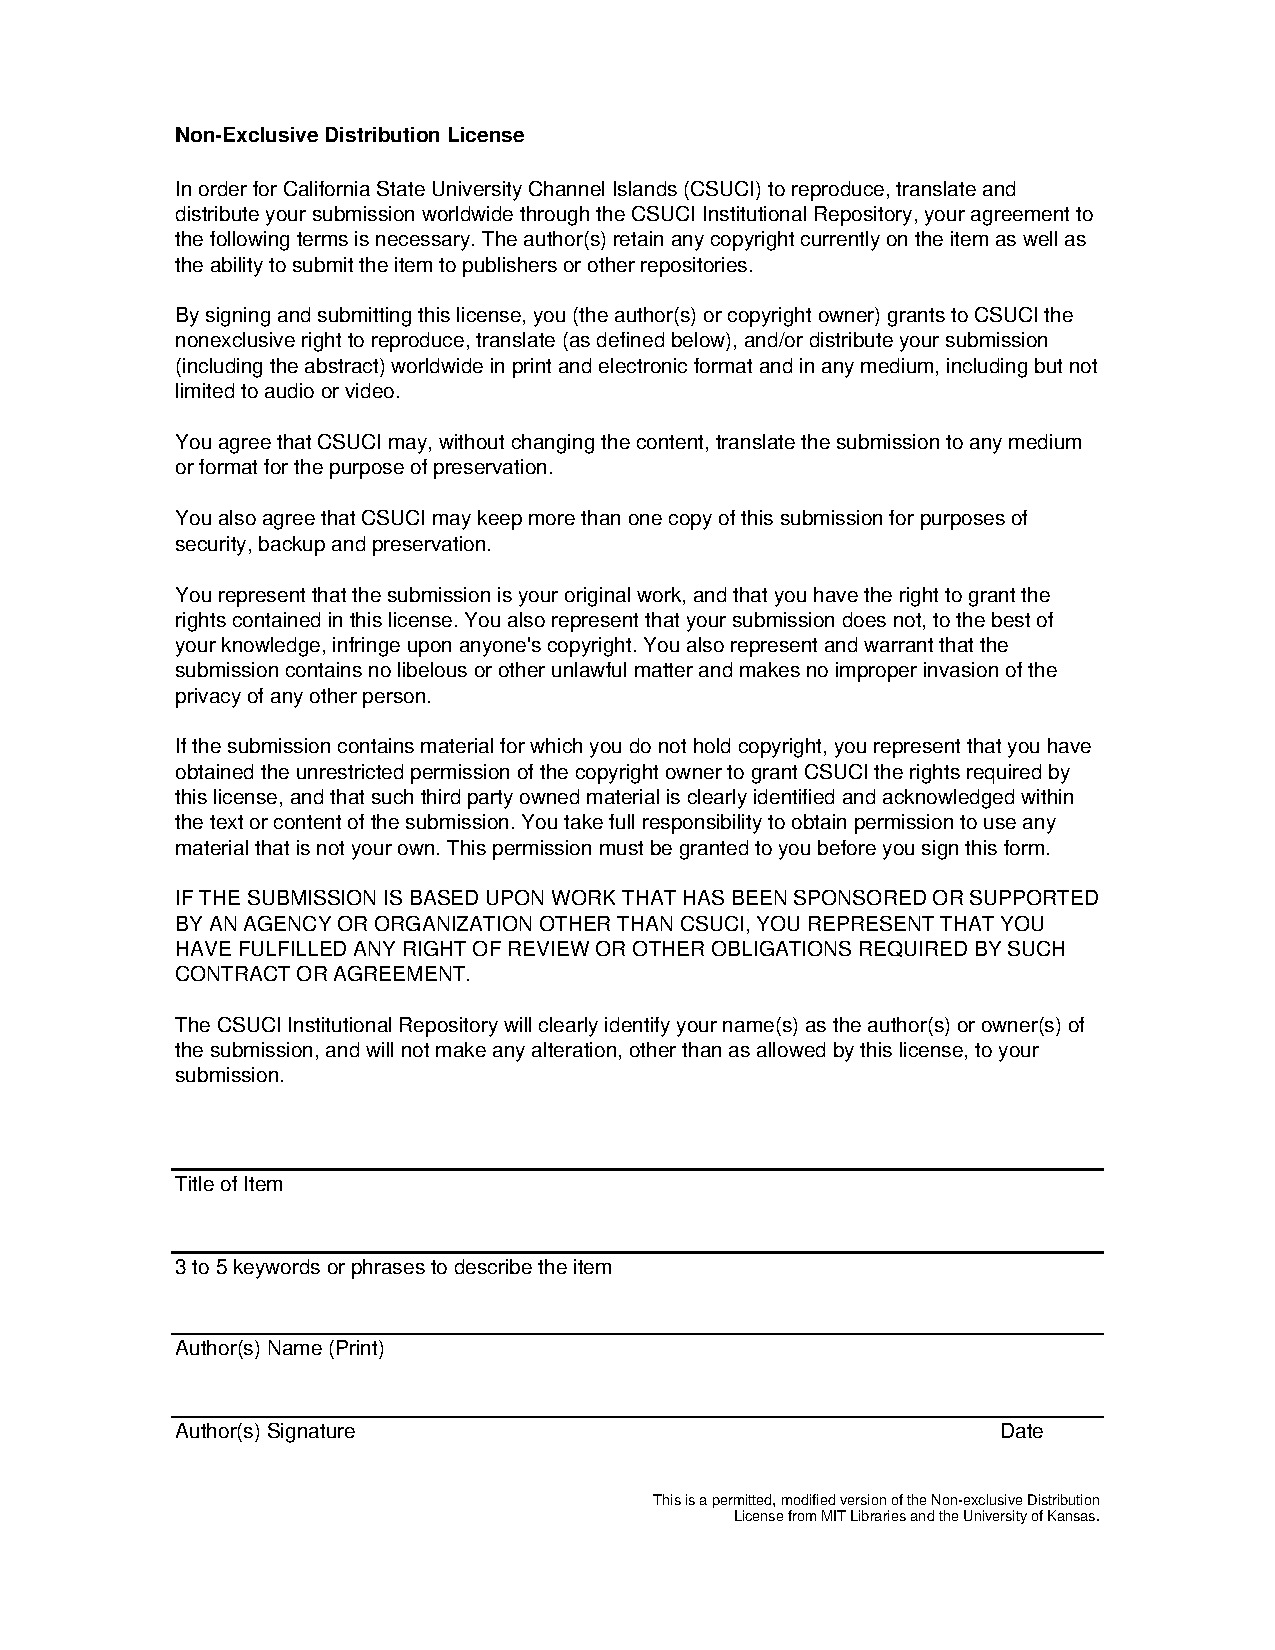
\includepdf{DistributionLicense.pdf}

\newpage

\title{SEAKER:\protect\\A Mobile Digital Forensic Triage Device} 
\author{Eric Elwood Gentry}

\date{\today}
\maketitle

\small{\textbf{Keywords}: Digital Forensics, Digital Forensics Triage, Mobile Digital Forensics,
Digital Evidence, Digital Evidence, Forensic Tools, \gls{rpi}}
\\

\begin{abstract}
As our world of digital devices continues to expand, the potential for digital evidence available to law
enforcement during case investigation is ever increasing.  The growing amount of digital evidence, along with
the deprived pool of Digital Forensic Investigators is causing a backlog to form at many of the digital
forensics labs around the world.  This backlog leads to delays in evidence analysis and reporting, causing
investigators and prosecutors to postpone or even drop on-going cases.\\

The \gls{seaker} device is a digital forensic triage tool that is designed to be simple, portable, inexpensive,
robust, and easy to use.  \gls{seaker} is an acronym for Storage Evaluator And Knowledge Extraction Reader.  
Utilizing a \gls{rpi}, this is a novel approach to helping provide immediate feedback to investigators
along with attempting to stem the backlog problem.  It was originally developed for on-scene investigations
that require immediate feedback, especially in time-sensitive investigations.  It also appears to be an
excellent tool to help reduce the backlog by preventing over-collection of digital evidence.  \gls{seaker} is not
meant to replace a fully-functional digital forensic lab, but instead to augment the initial investigation
and help reduce the backlog.  This research and device overview proposes the mobile, inexpensive, digital
triage device called \gls{seaker}.
\end{abstract}

\newpage
\pagenumbering{roman}

\tableofcontents

\newpage

\printnoidxglossaries

\newpage

\listoffigures

\newpage

\listoftables

\newpage
\pagenumbering{arabic}


\section{Introduction and Literature Review}
\label{sect-IntroAndLitReview}

\subsection{Introduction}
Law enforcement investigations involve many aspects of criminality and need carefully thought-out
procedures and practices.  These procedures and practices are essential to finding the evidentiary
information necessary to determine criminal liability, but are also in place to ensure that the evidence
collected is not tainted and is sound, viable, admissible court evidence.  Establishing and retaining the
forensic integrity of the evidence is a required and crucial part of the investigator's task.\\

Performing investigations is also a noteworthy endeavor.  There are many steps involved that require special
training to be performed properly.  One primary example is the {\em chain of custody}.  This refers to the 
step-by-step documentation record regarding evidence that includes details such as who had custody of
the evidence, when they had custody, who it was transferred to, who analyzed it, etc.
Another is the exacting
science of collecting, labeling, itemizing, and acquiring of evidence.
For instance, collecting physical evidence requires the
use of gloves,
evidence bags, fingerprint-dusting equipment, etc. to prevent cross-contamination, fingerprint smudging,
DNA evidence mishandling, and a multitude of other evidence tainting.  Without the proper adherance to 
guidelines,
even conclusive evidence may not be admissible during a case.\\

Digital evidence is also very essential to many investigations and cases in the modern world.
With each passing year, more and more digital devices are collecting, storing, and uploading data.  As
well, electronic devices for personal use appropriately labelled the Internet of Things (IoT) or
the Internet of Everything (IoE) are becoming more and more
ubiquitous in our everyday lives.  IOT devices are now everyday household items like refrigerators,
thermostats, light bulbs, window coverings, garage door openers, keys, clothes, and much more.
These devices and the massive amount of digital information that
is being generated and collected are often helpful in criminal investigations.  The data can be used to
construct timeframes of activity, locations of individuals, Internet activity, computer users and usages,
and lots other potential digital information.\\

One growing and particularly helpful aspect of an investigation is digital forensics.  This not only 
involves collecting potential digital evidence, but also analyzing, 
and reporting procedures.  This almost always requires a search warrant - a court-ordered search and
seizure of potential evidence of a location where a suspect resides, works, or may be storing it.
The search warrant is executed after it has been obtained from a judge and can involve physical and
digital evidence, as well as other items of consequence.\\

Search warrant investigations are often fraught with danger, intentional obscurity, hidden evidence, and
potential mishandling of evidence.  Before anything else can be done, the location must be considered
secure - considered safe from harming investigators and free of potential threats.  Once a scene is
secured at a search warrant service involving electronic evidence, three activities
take place simultaneously: the search for physical evidence, the search of the physical evidence
itself for electronic evidence, and the interviewing of involved parties.\\

The physical and digital evidence can guide the interviewing of the suspect(s), but also
has the potential to have both positive and negative effects on the
outcome of the investigation. If investigators do not locate any physical evidence for an examiner
to evaluate, then intelligence is not gathered and the interviewer has less information with which
to confront the suspect(s). If investigators present physical evidence to an examiner who is able to
evaluate it quickly in the field, then the interviewer (who is oftentimes also the lead investigator
on the case) can confront the suspects and potentially secure statements that lead to prosecution.\\

This leads to the need for digitial forensics specialists to bring their lab equipment into the field,
especially when serving a search warrant.  The lab equipment is specialized software and hardware
designed to analyze, report, and maintain forensic integrity on potential digital evidence.  This
equipment often involved a laptop, a write-blocking device, media imaging storage devices, expensive
software, and associated cabling for connection and power.  As well, this software is designed for
extensive and in-depth searching and often takes hours or days to analyze the evidence.  Many of the
reports from these systems are designed to be thorough and may take a skilled digital forensic
examiner days to pour over the material produced.  Oftentimes, this equipment is not brought
into the field and all digital evidence is simply collected for later analysis at the law
enforcement facilities.\\

The need for a more field-friendly digital forensic {\em triage} solution will assist in the initial
investigation tasks in multiple ways:
\begin{enumerate}
  \item It enforces a structured procedure and approach that is user-friendly to {\em non-digital
  forensic aware investigators} with the goal of simple instructions for use and very simple 
  evidence location.
  \item It enables investigators, especially interrogators, a very fast digital-evidence overview
  into the types of files
  and information being accessed and stored on the computer equipment at the site of the search
  warrant.
  \item It limits the number of devices and therefore the amount of data required in the in-depth
  analysis phase at the lab.
  \item It minimizes the impact and inconvenience to innocent parties at the site of the 
  search warrant.  The devices that are searched and found to have no evidenciary value can be
  deemed inconsequencial to the case and not be taken into custody.
  \item It may be used to provide initial, albeit simplified, analysis results on potential
  digital evidence ingested into the digital forensic lab.
\end{enumerate}

The topic explored in this paper is a portable, inexpensive, efficient device, named \gls{seaker},
that is intended
to overcome the need for a full digital
forensic lab equipment suite to be brought into the field.  The \gls{seaker} device was conceived and 
an initial prototype was produced at the California State University Channel Islands (CSUCI)
campus in a 
Masters level Computer Security class (COMP 524, Summer 2017) in direct collaboration with the
Southern California High Tech Task Force (SCHTTF) division of the Ventura Country
District Attorney's (VCDA) office.\\


\subsubsection{Author's Contributions}
Author's direct contributions to the \gls{seaker} device project:
\begin{enumerate}
  \item Developed the bash script to turn a standard \gls{rpi} into a
  \gls{seaker} device by programmatically
  installing raspbian software packages, setting up WIFI as a wireless access point, adding a web server,
  and preparing the running environment with the proper fileset
  \item Wrote a custom executable using the C programming language to increase the \gls{seaker} device's 
  searching efficiency in lieu of slower, native operating
  system solutions for finding content on digital media
  \item Co-presented and demonstrated the initial \gls{seaker} prototype for the Summer 2017 Masters level CSUCI
  Security class project to SCHTTF, CSUCI department heads, and local community leaders
  \item Presented the \gls{seaker} device as a thesis project at the April 2018 CSUCI Cyber Security Event
  to CSUCI President
  Erika Beck, California State Assembly Member Jacqui Irwin, Ventura County Sherriff's Department,
  and other local community leaders
  \item Co-authored a conference paper on the \gls{seaker} project and the technology behind it
  \item Updated and enhanced the \gls{seaker} device functionality to support the latest raspbian operating system (Stretch
  Lite, April 2018 release), including enabling ethernet passthrough to the wireless access point
  \item Co-authored by creating Logic Models and assisting with read-throughs for a United States
  Department of Justice (DOJ)
  grant proposal for future work on this project (\gls{seaker}) and
  a second, related security project (Voyager)
\end{enumerate}

\subsection{Literature Review}
\subsubsection{History of Digital Evidence}

The digital forensics field began in the mid 1980s with an understanding from several law enforcement
agencies that computers would play a critical role in future criminal investigations of the future.
In 1993, the FBI hosted an international conference on computer evidence in Virginia.  This was
the first major conference on the subject and had attendees from 26 different countries.  Much
of the original computer
forensics at that time related to recovering information from local computers.\\

Among the early pioneers in the digital forensics field, there was a common understanding that a
system of processes and procedures were needed to locate, record, analyze and report information.
This process would have to be similar to how non-digital physical evidence was handled, but also
include other computer specific preservation methods to ensure the integrity of evidence found.
Those processes and procedures have increased in complexity over time and have suffered from the
lack of unanimous adoption to a single standard.\\

In 2006, Rogers et al\cite{rogers2006computer} proposed a standardization model for a portion
of the entire process called {\em triage} for digital
forensic examiners to follow: Computer Forensics Field Triage Process Model.
The authors of the CFFTPM note the important legal and technical
considerations prior to implementing CFFTPM on a particular investigation.  The legal
considerations include issues
related to search warrant scope and its limitations, U.S. Constitutional 4th Amendment rights, etc.
The technical 
considerations include type of case, criticality of timeliness, skillset of the on-site
digital forensic examiner, 
skillset of the suspect, having proper lab equipment on-site, scene control, etc.\\

Even as late as 2013, Shaw et al\cite{shaw2013practical} points out that neither digital forensic
triage examination nor digital forensic full examination are well defined.
Digital forensic triage may mean something completely different to two digital forensic
examiners.  As well, full digital forensic examination has no robust standard to follow, Although
there has been no shortage of attempts.\\

The National Institute of Standards and Technologies (NIST) published guidelines for several
different types of digital evidence, for instance mobile phones, and computers.
However, NIST focuses on the analysis portion of the science, but leaves the collection,
and reporting aspects unexplored.  The International Standards Organization also published
a set of guidelines, but primarily focused on collection and handling aspects of digital
evidence.  
Ajijola et al\cite{ajijola2014review} provided a thorough review in 2014 of the NIST SP
800-101 Rev. 1:2014 guidelines
titled Guidelines on Mobile Devices Forensics and ISO/IEC 27037 titled
Guidelines for
Identification, Collection, Acquisition, and Preservation of Digital Evidence.
Their recommendation was a combined approach, though still not a fully formed solution.\\

\subsubsection{Process and Procedure Standardization}

Several approaches over the years have been proposed as universal processes and procedures to
gathering, reviewing, and presenting digital evidence.  These approaches range in number of
steps, process coverage, and overall methodology, 
but all have the common goal of finding usable digital evidence for preventing future
harm to society and preserving the potential digital evidence's 
integrity for means of presentation in court cases.\\

In the early years, some research facilities arose to help create and define the processes
and procedures necessary.  Among these were the Computer Analysis and
Response Team (CART), the Scientific Working Group on Digital Evidence (SWGDE), the
Technical Working Group on Digital Evidence (TWGDE), and the National Institute of
Justice (NIJ).  Since their respective inceptions, they have all strived and 
contributed to standardization on approaches and methods for 
the handling and processing of all digital evidence.\cite{noblett2000recovering}.\\

In addition, the United States Department of Justice (DOJ) published 
{\em Electronic Crime Scene Investigation: A Guide to First Responders}
\cite{ballou2010electronic} in the early 2000s that outlines
the necessary four steps for properly investigating digital Evidence:

\begin{enumerate}
  \item {\em Collection}, which involves searching for digital evidence,
  deciphering what should be collected, acquiring the media,
  and chain of custody documentation.
  \item {\em Examination}, which includes searching the digital media
  and attempting to reveal the evidence, especially when it is
  hidden or obscured.
  \item {\em Analysis}, intending to review the evidence for important
  legal infringements. 
  \item {\em Reporting}, for documenting the process used and evidence
  uncovered in the investigation.
\end{enumerate}

The 2003 {\em Integrated Digital Investigation Process} (IDIP)\cite{carrier2003getting},
proposed by Carrier, et al is a model that in their own words:
\begin{quote}
``uses the theory
that a computer is itself a crime scene, called the digital crime scene, and applies crime scene
investigation techniques.''
\end{quote}
It consists of five main phases (in addition, see figure \ref{fig:IDIP}):

\begin{enumerate}
  \item {\em Readiness}, for training, preparedness, infrastructure and resources
  preparation before any investigation even begins.
  \item {\em Deployment}, which is intended to capture the process for when an 
  incident requires digital evidence procedures and assignment of resources.
  \item {\em Physical Crime Scene Investigation}, for processing the physical
  evidence from the environment.
  \item {\em Digital Crime Scene Investigation}, for collecting and
  analyzing the digital evidence that exists in the virtual environment.
  \item {\em Review}, for examining the process used in the investigation and
  potential areas for improvements. 
\end{enumerate}

\begin{figure}[ht]
  \centering
    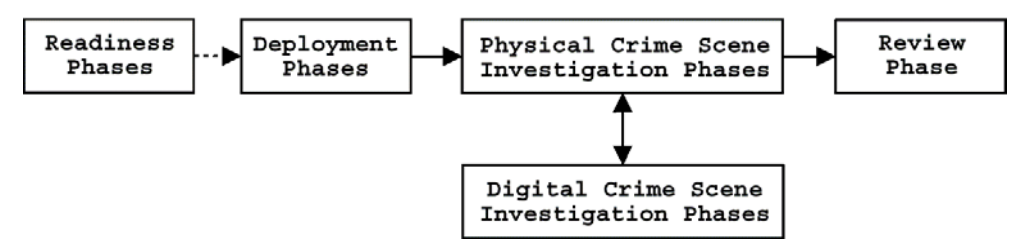
\includegraphics[width=0.8\textwidth]{images/IDIP.png}
  \caption{Integrated Digital Investigation Process Model (IDIP)}
  \label{fig:IDIP}
\end{figure}

Baryamureeba and Tushabe\cite{baryamureeba2004enhanced} proposed a model based
on the best parts of the US DOJ's {\em Electronic Crime
Scene Investigation}, the {\em Abstract Digital Forensics Model}, and 
the IDIP model.  Their proposal was called the
Enhanced Integrated Digitial Investigation Process (EIDIP).
Their model was proposed in 2004 at the annual Digital Forensic Research conference
(DFRWS)\cite{baryamureeba2004enhanced} and included the following phases:

\begin{enumerate}
  \item {\em Readiness}, same as IDIP.
  \item {\em Deployment}, which encompasses the Deployment,
  Physical Crime Scene Investigation, and Digital Crime Scene
  Investigation phases from IDIP.
  \item {\em Traceback}, that includes connecting the evidence collected
  in the previous phase to the suspect(s).  Typically this is done with IP
  addresses and requires the authority to gather this information.
  \item {\em Dynamite}, which includes the reconstruction of the events
  suggested by the evidence and  the documentation and submission to the
  appropriate legal authories.
  \item {\em Review}, same as IDIP.
\end{enumerate}

In 2006, Rogers et al\cite{rogers2006computer} proposed a reliable, repeatable process 
model designed specifically for digital evidence triage called
Computer Forensics Field Triage Process Model (CFFTPM). It was created in partnership
with Purdue University's Cyber Forensics and Computer and Information
Technology Departments, along with the National White Collar Crime
Center\cite{rogers2006computer}.
The process was derived from several other military and law enforcement models
including IDIP, 
Digital Crime Scene Analysis (DCSA),
and a military Operations Order (OpOrd).  In coordination with the Southern Indiana 
Assistant U.S. Attorney's office,
USADA Steve Debrota, Rogers et al\cite{rogers2006computer} implemented and reported
on the success of their proposal.  This amalgamation of approaches is still inspiring 
the latest trends in Digital Forensic approaches.\\

Shaw et al\cite{shaw2013practical} analyzed the ACPO and focused on the second step (Capture)
as the primary guideline for evidential integrity.  They strongly suggest compliance with
digital forensics best practices, like the ones provided in the ACPO.  Their final approach
and recommendation was to combine Linux utilities with a simplistic interface to standardize
the output and enable investigators who may not have full digitial forensic backgrounds
to perform triage on potential digital evidence.\\

The Association of Chief Police Officers (ACPO), a private company that helped establish and
develop policing practices in England, Wales, and Northern Ireland for many years,
put together a {\em Good Practice Guide for Digital Evidence}\cite{williams2012acpo} in 2012 that outlines some
recommended procedures for dealing with digital evidence.  As with other methodologies, this guide
explains utilizing a four step approach: Plan, Capture, Analyze, Present.\\

The ISO/IEC 27037 guidelines provide an attempt at an internationally 
recognized approach,
with the goal of making it easier to compare, combine, and contrast
results for out-of-jurisdiction cases and for data scientists' research.  It provides a
common reference line for 
digital forensics\cite{ajijola2014review}.  However, it is not meant to replace laws or regulations.
The main purpose is to provide practical
assistance for investigations involving potential digital evidence, while preventing digital
evidence corruption.  This
process facilitates the usability of evidence by other jurisdictions.  This guideline provided
four steps for handling
potential digital evidence: Identification, Collection, Acquisition, and Preservation.  However,
this is incomplete, as
it only addresses gathering, not actually evaluating or providing results to law enforcement
investigators.\\

All of these approaches are intended to help find and gather digital evidence.  They are also intended
to maintain the forensic integrity.  Some organizations combine these approaches into a system of
processes and procedures intended for use in their own facilities.  Unfortunately, many organizations have
home-grown solutions passed down from senior members of the digital forensics team to the newer
team members.  Not having a universally recognized and accepted standard 
leads to complications and difficulties when digital evidence needs to be shared across other
jurisdictions and boundaries\cite{ajijola2014review}.\\

\subsubsection{Aquisition Methodology}

[MOVE THIS TO THE NEXT CHAPTER!!!!]
The \gls{seaker} tool is designed specifically for the {\em triage} phase of digital forensic
investigations.  As a general approach, this research splits the act of dealing with digital evidence into two
separate methodologies: {\em aquisition} and {\em analysis}.  These are the main foci since \gls{seaker} is 
designed to do both in a very timely fashion and are the main focus of this research.\\

Aquisition has multiple definitions across
the digital forensic universe, but in this case it is meant to imply the entire set of processes and
procedures from training the digital forensic examiners and \gls{seaker} users,
to collecting the media that potential digital evidence may be stored on, 
to the \gls{seaker} usage for gathering the information about each device.\\

The aquisition phase specifically highlighted here is the gathering of physical digital
media and the capturing of potential digital evidence in the triage environment.  The 
setup and training materials for creating and using the \gls{seaker} device are referenced in
the appendix.\\

The analysis step will be discussed in the next section.\\



\subsubsection{Analysis Methodology}

The {\em Analysis} methodology is considered the second phase in the \gls{seaker} approach and 
can consist of both the {\em triage} analysis stage and the {\em full} analysis stage.
Specifically, this paper and the \gls{seaker} device focus on the triage stage of Analysis.  This
stage can be applied in the field or at the digital forensics lab, while the full analysis
is unlikely to be accomplished in the field.  A full analysis could take many hours or days
and is not the first priority when serving a search warrant.\\

However, digital evidence triage is a very useful part of an investigation and can be 
implemented using the \gls{seaker} device.  The triage analysis stage is considered in this research
to consist of an interactive web page that detectives and investigators can use to 
lookup search terms from the digital evidence collected from suspect devices plugged into the
\gls{seaker} device.\\

Rogers et al\cite{rogers2006computer} research in 2006 covered the primary machine type at
the time: the standard Windows machine.  Unfortunately, this leads to an outdated model over
time, since the processes and procedures become obsolete as new technology arises.  Along with
the proliferation of IOT devices, new technologies also have emerged as more mainstream that
need to be incorporated into a more generalized approach.  Some operating systems are being
utilized on a more regular basis, like Linux and Mac.  In fact, even our \gls{seaker} device is
an IOT device based on the unix spin-off of Debian.\\

Ajijola et al\cite{ajijola2014review} - The NIST guidelines provide an in-depth look into mobile
devices, helping to explain the technology involved and its
relationship to the forensic process.  NIST itself is a technological, non-regulatory federal agency under the U.S.
Department of Commerce.  The NIST process model labeled NIST SP 800-101 lays out the digital evidence procedures in
four steps: Preservation, Acquisition, Examination and Analysis, and Reporting.  These four steps provide the
necessary steps for the digital evidence process model as a suggested way to evaluate mobile device information.  This
is useful, but not complete for law enforcement investigators.\\

\subsubsection{Combined Aquisition and Analysis Methodologies}
Hitchcock et al\cite{hitchcock2016tiered} has proposed and evaluated a ``tiered forensic methodology'' model that defines
a process of digital forensic triage utilizing non-digital evidence specialists.  In their research, they identified
a large and growing backlog of digital evidence.  This backlog has led to problems in the law enforcement community
with regards to collecting, analyzing, reporting, and prosecuting.\\

The next tier is when the already-triaged digital evidence is sent for full evaluation.  This is a certified facility
that can perform full digital forensic analysis, called a Technological Crime Unit (TCU).  The TCU is currently
heavily inundated with cases needing analysis and reporting of digital evidence.\\

This tiered approach is based on a Computer Forensic Field Triage Process Model proposed by Rogers et al
\cite{rogers2006computer} and the internation standard ISO 27037 (Information Technology - Security Techniques - 
Guidelines for identification, collection, aquisition, and presentation of digital evidence). The process model 
breaks down the six phases of digital evidence categorization, which Hitchcock et al\cite{hitchcock2016tiered} loosely
based their four phase approach on.  The four phases are: planning, assessment, reporting, and threshold.  The ISO
27037 standard specifically attempts to address the need to minimize the risk of potential digital evidence being
spoiled by mishandling, while also attempting to maximize the evidentiary value of digital evidence collection.\\

This approach is not without risks.  One concern is the accidental exclusion of an item of digital evidence that is
important to the investigation.  Another is the level of computer skills and training of the DTF expert.  The paper ???
does attempt to mitigate the latter with training and management process, while providing evidence that the former
is a common misconception in most cases.\\

Shaw - One example is to note encrypted compressed files for review later.\\

Rogers - This process in no way supersedes the ability or need to perform a full forensic examination at a full-featured
digital forensic lab.\\

Ajijola et al, 2014\cite{ajijola2014review} also proposed a new process
model that is a hybrid of both models with the resulting combination being much more effective than either of its 
individual parts.\\

In the research for combining the NIST and ISO guidelines, Ajijola et al\cite{ajijola2014review} explores the
commonality, differences, and limitations of each model.  Although both models follow the Auditability,
Repeatability, Reproducability, and Justifiability requirements, as well as the Confidentiality, Integrity, and
Availability standards, they individually lack some necessary phases to enable them to be used separately.  The NIST
process model lacks the Identification and Collection phases, while the ISO process model lacks Examination, Analysis,
and Reporting aspects of a full Digital Evidence processing model.\\

The combination of these two approaches, as suggested by Ajijola et al\cite{ajijola2014review}, provides a new five 
step approach: Identification, Collection and Acquisition, Preservation, Examination and Analysis, and Reporting.
These steps provide a more comprehensive approach that law enforcement can use to fulfill its evidenciary duties in
an investigation.  When both process methods are used, the goals approach a full set of tasks from initial on-scene
evalutation to the end of the in-lab digital forensics investigation.\\

\subsubsection{Digital Evidence Backlog}
IDC forecasts that by 2025 the global datasphere will grow to 163ZB (see Figure 1) (that is a trillion gigabytes).
That's ten times the 16.1ZB of data generated in 2016. All this data will unlock unique user experiences and
a new world of business opportunities.\\

\begin{figure}[ht]
  \centering
    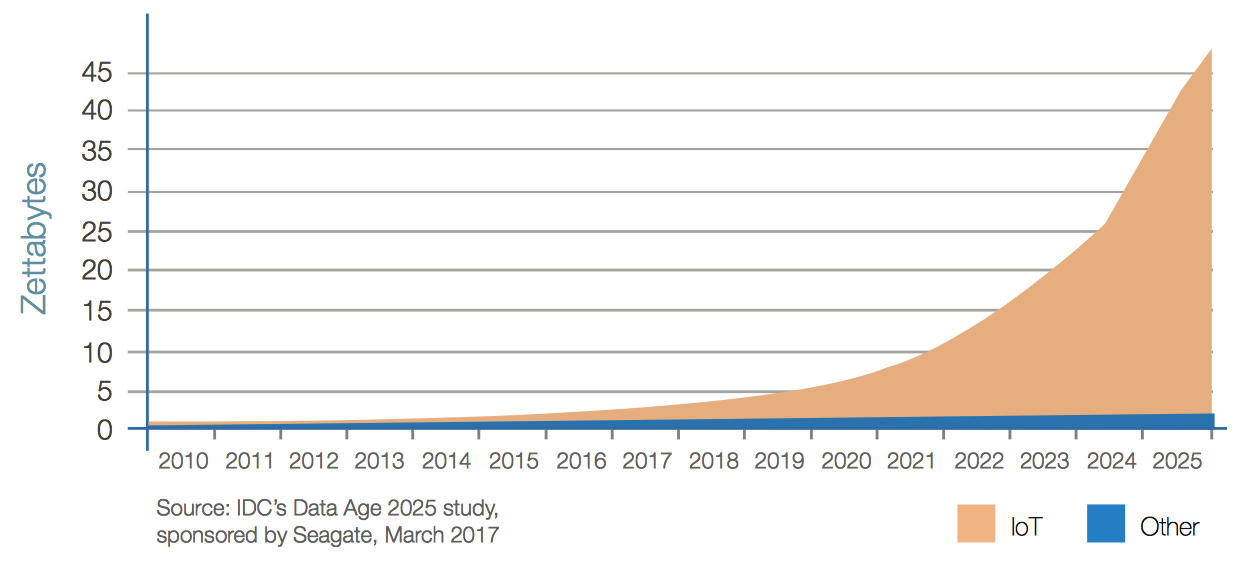
\includegraphics[width=0.8\textwidth]{images/IOT_chart.jpg}
  \caption{IOT Device Data Growth}
\end{figure}

Some of the current challenges in digital forensic investigations are directly related to the amount of data being
created.  As Lillis et al\cite{lillis2016current} explores in their research, there are three main factors
involved in the digital forensic backlog: increasing number of devices seized per case, increased number of cases
involving digitial evidence, and the increasing volume of data per digital media.  This has lead to a growing
and already substantial backlog in digital forensic investigations.\\

One effect of this increased delay and backlog is that cases become inactive, waiting for new leads.  A more
aggressive approach to solving the backlog could help prevent dismissals, cold cases, and potentially more
societal harm from a corrupt investigation suspect.\\

Raghavan\cite{raghavan2013digital} has accumulated a list of 5 major challenges that the digital forensics 
community is facing and continue to add to the backlog problem.\\

The first is the complexity of binary data aquisition, i.e. low level data aquisition through digital media
duplication.  This challenge causes the need for sophisticated data reduction techniques.\\

Another complexity is the diversity of data and lack of standard examination techniques.  The plethora of
operating systems and file formats has been increasing and is posing a more and more significant challenge
over time.\\

The consistency and correlation problem is yet another challenge.  This is a problem resulting from the current
digital media investigation tools not providing the entire picture to investigators.  Only part of the whole
picture is provided when these tools find digital evidence.\\

Another issue that Raghavan\cite{raghavan2013digital} proposed is the volume of data to sort through.  The sheer
amount of data that exists per user is increasing at an alarming rate [cite?], and has lead to a very large
backlog of digital evidence to investigate.  These delays have even caused some cases to be dismissed.  This
challenge is exacerbated by the lack of adequate automation for digesting the data.\\

The fifth, but certainly not the last, challenge proposed by Raghavan\cite{raghavan2013digital} is the timeline
synchronization issue with digital evidence.  Since the evidence could be collected in different time zones, 
with different timestamp formats, clock skew, etc, lining up the events in order can be challenging or
infeasible.\\

With the proliferation of Internet Of Things (IOT) devices and cloud storage, the field of digital forensics
continues to expand.  These areas pose a great challenge, but also new opportunities.  Lillis et
al\cite{lillis2016current} researched cloud storage and found some areas of opportunity, for instance parallel
processing, distibuted computing, GPU/FPGA utilization, and others.  These areas for increasing the efficiency
of ditigal forensics can be explored further due to the substantially reduced I/O limitations in cloud storage.\\

The Internet of Things (IOT) also poses new challenges.  IOT devices are estimated to number near 40 billion by
2020, contributing to the overwhelming amount of digital data.  Since these devices tend to have more 
non-persistent memory and less storage, this causes added complexity for gathering and analysis.  In addition,
a portion of IOT devices are battery operated and computationally challenged, leading to loss of data over
time.\\

Hitchcock et al\cite{hitchcock2016tiered} - The backlog and delays in case reporting are contributors to a common problem of time sensitivity.  Some countries 
have given their citizens a right to a ``speedy'' trial.  As well, some countries have statutes of limitation (limits
on how long after the crime was committed to resolve the case) for most crimes.  Some administrative situations are
also contributors, for instance case prioritization based on chronological filing, crime severity, or victim needs.\\

\subsubsection{Digital Evidence Triage}
The summary of the research done by Hitchcock et al\cite{hitchcock2016tiered} are as follows.  They sought to expedite
the process of sending digital evidence for analysis and results.  One of their goals is to enable more field triage
of digital evidence to reduce the amount collected, and act specifically on pertinent information only.  They 
recommended that some front-line crime scene investigators (non-forensic analysts) be trained in the implementation
of digital evidence triage and evaluation.  These trained individuals would be Digital Field Triage (DTF) experts and
have the ability perform field-level digital evidence triage.  This triage would specifically weed out the benign
from the consequential digital evidence with high certainty, while also protecting the digital evidence from spoilage
and preserving evidentiary integrity.\\

One digital evidence triage method proposed by Shaw et al\cite{shaw2013practical} seeks to standardize on an 
approach they call ``enhanced previewing''.  Enhanced previewing seeks to solve some of the problems associated with
typical triage approaches.  As is the case in other research, Shaw et al\cite{shaw2013practical} extolls the 
need to reduce digital forensic evidence analysis backlogs, especially with the evolution of big data and the
proliferation of digital devices.\\

The proposal for a practical and robust methodology by Shaw et al\cite{shaw2013practical} aims to stem the concerns
of a typical triage process.  Risks still exist, for instance overlooking digital evidence, but it is argued that
those risks are outweighed by the risks of a lengthy process due to large backlogs and the associated delays in
evaluating that evidence.  Another concern exists that inadequately trained people will be charged with performing
on-site digital evidence triage and mishandling or incorrectly evaluating results will cause evidence spoilage.
Other concerns are the potential high cost of software and training.\\

In order to provide a simple, yet robust mechanism, Shaw et al\cite{shaw2013practical} starts with an open source,
CD-bootable image of GNU/Linux and enhances its features to include boot-time application launching, and a simple
to use interface with minimal ability to deviate from task.  This bootable CD is intended to be placed into 
evidenciary computer systems and booted using a series of BIOS modifications or boot-time interruptions.  This 
mechanism to boot the system off of a bootable CD is difficult, and where the most problems with untrained users
of the enhanced previewing will happen.\\

The enhanced previewing concept has valuable merit, in that the collection mechanisms are thorough.  Using the
GNU/Linux based system and having written code for it, Shaw et al\cite{shaw2013practical} utilized some well
thought-out approaches.  First, all hard drives from the evidentiary system are mounted into the GNU/Linux
filesystem as read-only, thereby eliminating the need for write-blockers.  As well, the entire hard drive is
evaluated, including the file system, all partitions, unallocated space, deleted files, and compressed files.  In
addition, other mechanisms are employed that continue to enhance the previewing are employed.\\

Rogers - The CFFTPM was created to enhance the investigators ability to obtain useful information at execution time of a 
warrant at the suspect's dwelling or work.  The process is designed to be used in the first few hours of the 
investigation, especially during the first suspect interview and search execution phase of the investigation.  It is
known that suspects are more likely to divulge more information and be more cooperative in that environment (Yeschke
2003\cite{yeschke2003art}).  As well, location of and presentation with suspect ``triggers'' from the potential evidence
increase the suspect's willingness to talk and cooperate while on site.\cite{rogers2006computer}\\

The foci of the CFFTPM are immediately finding usable evidence, identifying victims at acute risk, guiding the
on-going investigation, identify potential charges, and accurately assess the offender's danger to society.\\

Rogers - The CFFTPM is broken up into phases, two of which have sub-phases (see Figure 2).  The main phases consist of Planning, Triage,
Usage/User Profiles, Chronology/Timeline, Internet Activity, and Case-Specific Evidence.   Usage/User Profiles are broken down into three sub-phases:
Home Directory, File Properties, and Registry.  These are important and help distinguish user specific activity and
permissions.  The Internet Activity phase is also broken down into three sub-phases: Browser Artifacts, Email
Artifacts, and Instant Messenger Artifacts.  These also help establish user activity.  Some importance is explicitly
stated to skip based on type of investigation and prioritizing the investigation.\\ 

\begin{figure}[ht]
  \centering
    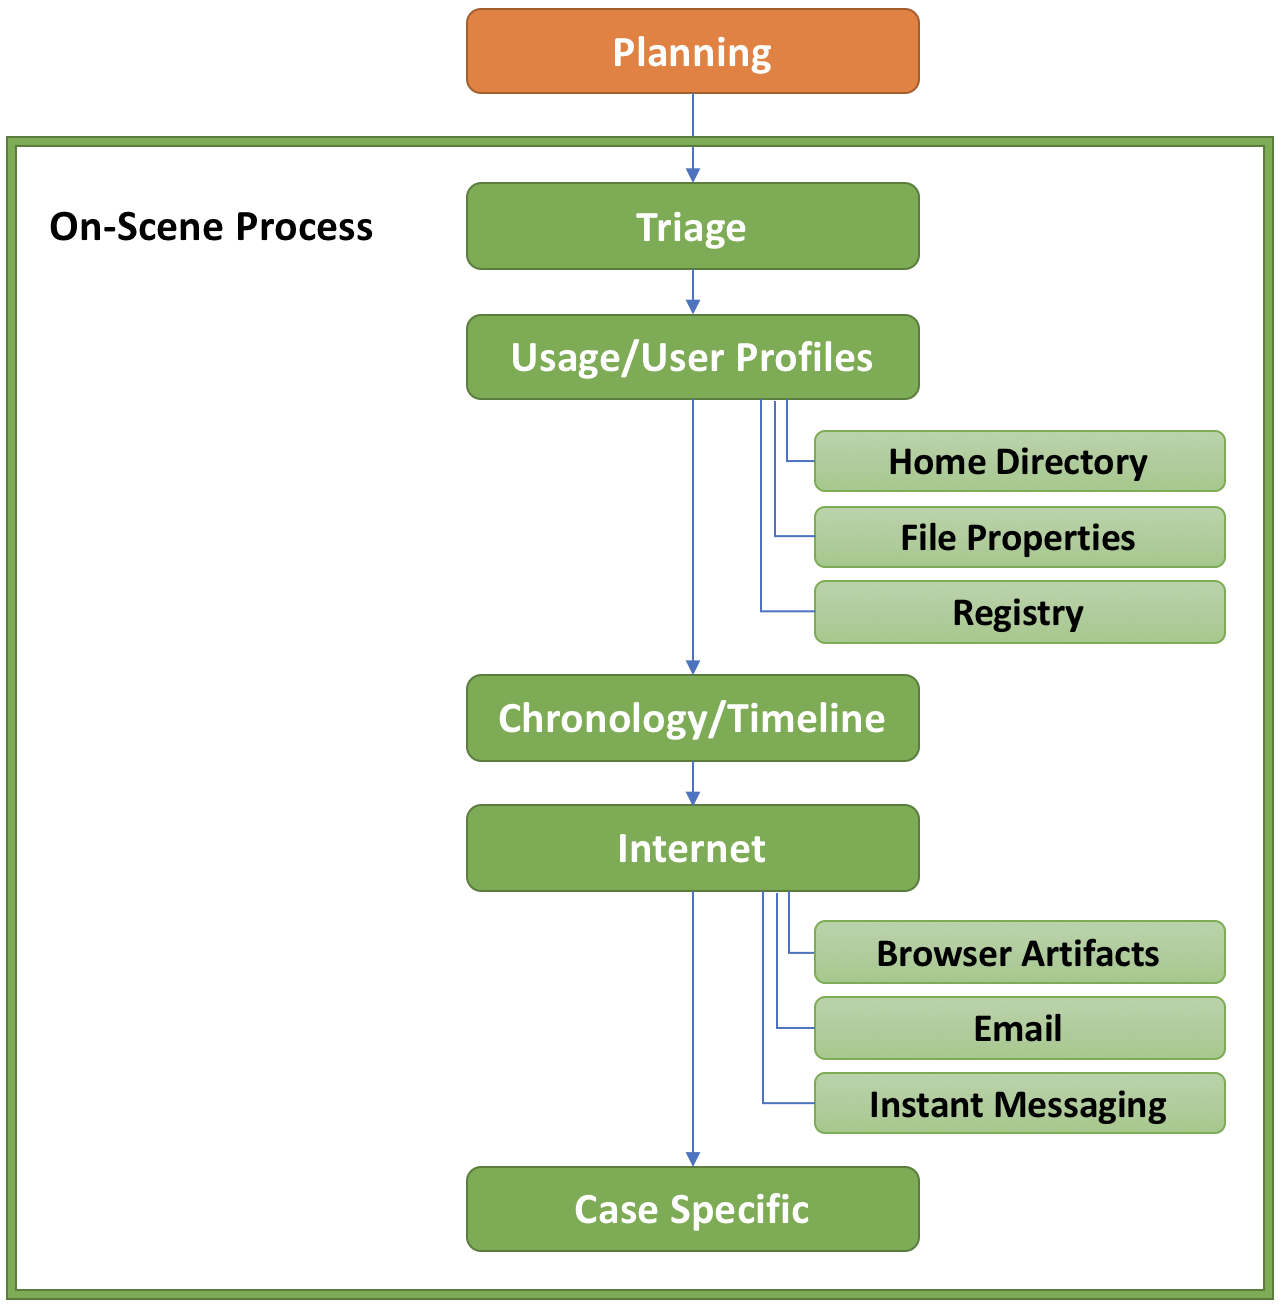
\includegraphics[width=0.8\textwidth]{images/CFFTPM.png}
  \caption{Computer Forensic Field Triage Process Model (CFFTPM)}
\end{figure}

\subsubsection{How \gls{seaker} Can Help}
The research of Hitchcock et al\cite{hitchcock2016tiered} should be referenced for a good process starting point for
digital forensic labs.\\

Rogers -  This is where the \gls{seaker} portable
triage device can help by evaluating every aspect and prevent the on-site investigators from skipping or
de-prioritizing critical potential evidence.\\

Rogers - This is also an area where the
\gls{seaker} portable triage device can help eliminate some of the potential problems, for instance technical prowess of the
on-site investigators and proper lab equipment on-site.\\

Rogers (CFFTPM) - Some particular aspects of the phases are critical to investigators in revealing evidence or potential evidence for
the \gls{seaker} portable traige device.  Usage/User Profile information is extremely important.  This includes the need to
be able to view and search files, folders, registry keys, and file properties associated with a particular user.  The
Internet Activity artifacts also become very useful, especially in the case of child pornography.  The browser, email,
and Instant Messaging artifacts can lead directly to potential charges.  Finally, a Chronology/Timeline understanding
and ability to sort based on it can significantly narrow down the possibilities of which user information and which
Internet Activity is the most important and critical to the investigation.\\

Rogers (CFFTPM) -Implementing this in the \gls{seaker} portable triage device is crucial for simplicity and ease of use.  As well, it goes a
long way towards having an implementation of \gls{seaker} being understood and adopted.  Reporting is also a critical need
and is implemented in a way that will enable digital forensic investigators to provide early information to
investigators and prosecutors.  This helps alleviate the need to wait until the backlog of digital evidence is cleared
to get any information from case-specific digital evidence.\\


\section{Background}
\label{sect-background}

In a labratory environment, digital forensics investigators have the ability to discover
a tremendous amount of material that is potential evidence.  This includes anything 
digitally stored on the evidentiary media from
explicity illegal files to IP address connections to a digital chronology of
events.\cite{raghavan2013digital}\cite{rogers2006computer}
The software and hardware necessary to perform the
in-depth, full evaluation of the media are specialized for digital forensics 
work, but typically are costly, don't travel well, and can take many hours for
results from a single digital media device.\\

In the field environment, digital forensics
investigators are likely to not have the time, equipment, or proper environment to
obtain evidence from the digital devices found during the execution of a search
warrant.  In some cases, due to various reasons, digital forensics investigators
are not able to attend and therefore all of the digital media is taken into
custody for analysis at the digital forensics lab.  When they are able to attend,
they typically
bring a subset of their lab environment with them to start deciphering
the digital information and attempt to perform a traige analysis.\\

In a coordinated effort with SCHTTF, this research is an attempt to help
solve some of the field environment limitations of digital forensics investigators.


\subsection{Legal Necessity and Implications}
Search warrants are necessary for 

write blockers
chain of evidence
\subsection{Technical Necessity and Implications}
\gls{rpi}
Cost 
human expertise
DEFR, DES, Digital Forensic 



\section{Development of \gls{seaker} Device}
\label{sect-developmentSeakerDevice}
great novelty
collaboration with industry HTTF
\subsection{Conception}
Masters Security class
SCHTTF project proposal
collaborated with SCHTTF
\subsection{Setup Script For \gls{rpi}}

\subsection{Rules For Mounting}
mention write blockers from chapter 2
\subsection{Code for Searching Device}

\subsection{Tools Used for Development}


\section{Experimental Results}
\label{sect-experimentalResults}

\subsection{Prototype Demonstration}
in-class example at end of semester
\subsection{Results}
graph of latency
estimates of time vs data Gb
examples of running on Frank disks


\section{Conclusions and Future Work}
\label{sect-conclusionAndFutureWork}


\section{Appendix}
\label{sect-Appendix}

\subsection{\gls{seaker} Setup}
The following set of instructions will detail how to setup the \gls{seaker}
environment for the first time. There are three install options that
enable \gls{seaker} creators to prepare the device.  See
Table~\ref{tab:RequiredSoftware}

\begin{enumerate}
  \item {\em Router}: This option is where the \gls{rpi} and the
  secondary computer are connected directly to the same router, thus
  allowing the same local DHCP to assign the IPs of both.  The
  secondary computer is used to prepare the micro SD card and to later
  remotely and securely connect to the \gls{rpi} to complete the
  setup.
  
  \item {\em Direct Connect}: This option is where the Raspeberry Pi
  is connected directly to a monitor and keyboard to enable direct
  user input via the termnial.  The secondary computer is necessary to
  prepare the micro SD card, but not used to remotely connect to the
  \gls{rpi} to complete the set up.

  \item {\em Corporate LAN}: This option is almost identical to the
  {\em Router} option, but utilizes a corporate network instead of
  a local router to connect to the \gls{rpi}.  This option is the
  most IT intensive, since the IP address assigned to the Raspberry
  Pi is often not easily found.
\end{enumerate}

\begin{center}
  \begin{tabular}{l|l|l}\hline\hline
    {\bf Option 1}    & {\bf Option 2}         & {\bf Option 3} \\
    {\bf (Router)}    & {\bf (Direct Connect)} & {\bf (Corporate LAN)} \\\hline\hline
    \multicolumn{3}{c}{}\\
    \multicolumn{3}{c}{Hardware Required} \\
    \multicolumn{3}{c}{}\\\hline
    & & \\
    \textbullet \gls{rpi} & \textbullet \gls{rpi} & \textbullet \gls{rpi} \\
    \textbullet Mac or Windows Computer & \textbullet Mac or Windows Computer & \textbullet Mac or Windows Computer\\
    \textbullet Micro SD card & \textbullet Micro SD card & \textbullet Micro SD card\\
    \textbullet Router & \textbullet Monitor\\
    & \textbullet Keyboard\\
    & & \\\hline
    \multicolumn{3}{c}{}\\
    \multicolumn{3}{c}{Software Required} \\
    \multicolumn{3}{c}{}\\\hline
    & & \\
    \textbullet Raspian Stretch Lite & \textbullet Raspian Stretch Lite & \textbullet Raspian Stretch Lite \\
    \textbullet ssh client & \textbullet ssh client & \textbullet ssh client\\
    \textbullet Disk Imaging software & \textbullet Disk Imaging software & \textbullet Disk Imaging software\\
    \textbullet IP Scanning software & & \\
    & & \\\hline
  \end{tabular}
  \captionof{table}{\gls{seaker} set up: Required Hardware and Software}\label{tab:RequiredSoftware}
\end{center}

The following creation process is required to setup the \gls{seaker} device
to the specifications outlined in this paper.  Figure~\ref{fig:SeakerCreation} 
outlines the general process, while the specific steps are listed below.

  \begin{figure}[ht]
    \centering
      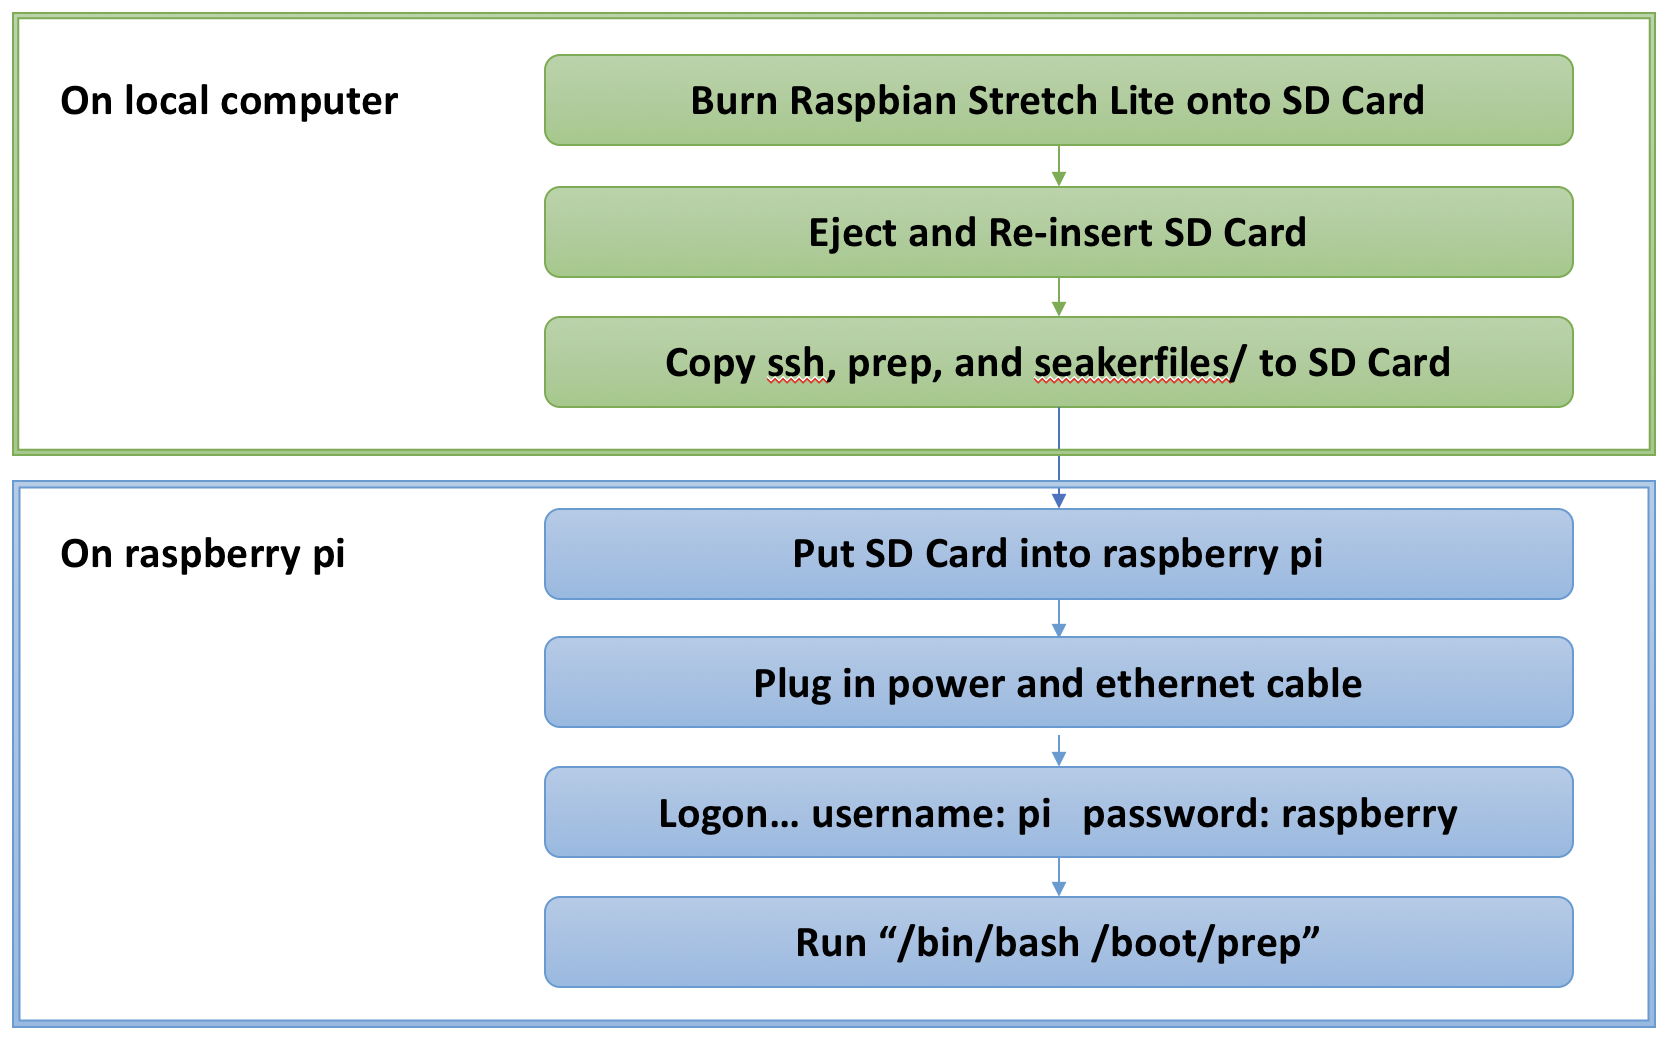
\includegraphics[width=0.8\textwidth]{images/SeakerCreation.png}
    \caption{\gls{seaker} Creation Process}\label{fig:SeakerCreation}
  \end{figure}

\newpage

\begin{enumerate}
  \item Download the latest Raspbian Stretch Lite operating system\\
  (https://www.raspberrypi.org/downloads/raspbian/).
  Note the location where file is saved.
  \item Download the most recent copy of {\em prep.sh}, {\em ssh}, and the 
  folder called {\em seakerfiles}. These files
  contain \gls{seaker} setup and running code.
    \begin{itemize}
      \item prep.sh file location: https://s3-us-west-2.amazonaws.com/seaker/prep.sh
      \item ssh file location: https://s3-us-west-2.amazonaws.com/seaker/ssh
      \item seakerfiles location: https://s3-us-west-2.amazonaws.com/seaker/seakerfiles
    \end{itemize}
  \item Open prep.sh and edit the default configuration information
  (shown below). At minimum it is recommended to change the Raspberry
  Pi and WiFi passwords.

  \lstinputlisting[language=bash]{code/config.sh}

  NOTE: It is recommended to change the WIFI Name and IP Address when
  setting up multiple \gls{seaker} environments over time to ensure each
  environment has unique identifying information.\\
  \\
  For example: If setting up three \gls{seaker} environments, configuration could be:
    \begin{enumerate}
      \item Name: SEAKER01, IP Address: 192.168.101.1
      \item Name: SEAKER02, IP Address: 192.168.102.1
      \item Name: SEAKER03, IP Address: 192.168.103.1
    \end{enumerate}
  \item Insert micro SD card into computer (not the \gls{rpi}).
  An adapter will likely be required.
  \item Open disk imaging software (Etcher for Mac, or SDFormatter and 
  Win32 Disk Imager for Windows).
  Map to the Raspbian Stretch Lite file
  location, choose the micro SD card as the destination, and select to burn
  the image. (Refer to the chosen imaging software documentation for
  specific instructions on using this tool.)  Do not remove the micro SD
  card from the computer.
  \item Map to the micro SD card (Finder for Mac, File Explorer for Windows).
  Copy ssh, prep.sh, and the seakerfiles folder onto the micro SD card's
  {\em boot} partition.
  \item Remove the micro SD card from the computer.
  \item Insert the card into the \gls{rpi}.
  \item Power on the \gls{rpi} by plugging it in with the power cord.
  \item Identify the local IP Address of the \gls{rpi}:\\
  If installing with Option 1 (router):
    \begin{enumerate}
      \item Plug the \gls{rpi} into the same router being used by the
      Windows or Mac computer.
      \item Use the IP Scanning tool on the computer to find the local IP
      Address of the \gls{rpi}. The Manufacturer should be ‘Raspberry
      Pi Foundation’.
    \end{enumerate}
  If installing with Option 2 (Direct Connect):
    \begin{enumerate}
      \item Connect the monitor and keyboard to the \gls{rpi}.
      \item Login using the default username (pi) and password (raspberry).
      \item Enter the following command to retrieve the local IP Address:\\
      \begin{verbatim}
        ifconfig eth0
      \end{verbatim}
    \end{enumerate}
  If installing with Option 3 (Corporate Network):
    \begin{enumerate}
      \item The MAC Address of the \gls{rpi} is required. This can be
      located on the original \gls{rpi} box.
      \item For Windows systems, open a command prompt and enter the command
      below. Replace the ``c8:26:3b:d2:63:d5'' sequence with the MAC Address
      of the \gls{rpi} being configured.  Use the following command:
      \begin{verbatim}
        arp -a | findstr "c8:26:3b:d2:63:d5"
      \end{verbatim}
      \item For Unix or Linux systems such as Apple or Ubuntu, open a terminal
      window and enter the command below. Replace the ``c8:26:3b:d2:63:d5''
      sequence with the MAC Address of the \gls{rpi} being configured.
      Use the following command:
      \begin{verbatim}
        arp -a | grep "c8:26:3b:d2:63:d5"
      \end{verbatim}
    \end{enumerate}
  \item If installing with Option 1 or 3:
    \begin{itemize}
      \item SSH into the \gls{rpi} from the laptop or desktop computer.
      \begin{itemize}
        \item If using a client such as Putty, enter the local IP address
        of the \gls{rpi}, choose SSH and connect. Click \verb|OK| or
        \verb|Yes| on the security warning.
        \item If using a command line utility such as Bash enter the
        following at the prompt:
        \begin{verbatim}
          ssh pi@<ip_address> -l pi
        \end{verbatim}
        \item Login using the default username (\verb|pi|) and password
        (\verb|raspberry|).
      \end{itemize}
    \end{itemize}
  \item Run the preparation script by typing the following on the command line:
  \begin{verbatim}
    /bin/bash /boot/prep.sh
  \end{verbatim}
  \item Wait for the \gls{rpi} to finish running the script and
  rebooting. The \gls{rpi} should now be configured as a \gls{seaker}
  and be up and running.
\end{enumerate}

\newpage
\subsection{\gls{seaker} Usage}
After collecting all the media devices at the scene, the investigator
will triage them with \gls{seaker}. Here are the steps:\\

(1)~Connect the RP to the power and wait for about a minute
to let it finish booting up.
Connect to the RP's Wireless Access Point (WiFi network). Depending
on the setup, the WiFi's SSID will be ``SEAKER01'' or ``SEAKER02''
etc.  See Figure~\ref{fig:screen-1}. Note that \gls{seaker}'s Wireless Access
Point is password
protected and matches the one specified in the prep.sh script file.\\

\begin{figure}[ht]
  \begin{center}
  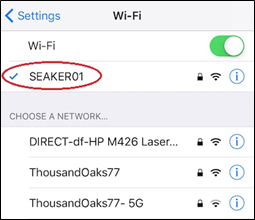
\includegraphics[width=4cm]{images/seaker-hh-screen-1.jpg}
  \caption{iPhone WIFI connection to the \gls{seaker}.}\label{fig:screen-1}
  \end{center}
\end{figure}

(2)~At the same time the investigator may connect all the media
devices to the RP. This may be done concurrently with the previous
step. Note that in order to examine a digital media it will need to be
removed from the
computer, and connected to the RP; this may be done through a
write-blocker interface but it is not necessary.\\

(3)~Once connected to the \gls{seaker}'s Wireless Access Point,
the investigator will open any
web browser on their connected device and direct it to go to
\verb|http://seaker01.local|. Access is allowed
through a web browser, as this is the most universal way to connect
on any device (iPhone, iPad, Android, laptop, etc.).  These
devices and many more can connect to a Wireless Access Point
and open a browser.  Once the browser establishes the
connection, the user will see Figure~\ref{fig:screen-2}. Note that the
keywords (or regular expression patterns) present in the ``Type in
Search Terms:'' can be pre-loaded before arriving at the scene, or
changed/updated at the scene.

The regular expression can be given using the syntax of the
\verb|grep| utility. For example, if we want to find occurrences of
either `two' or `too', we use \verb|t[wo]o|; if we want to find every
word that start with capital letters, we use \verb|^[A-Z]|; if we want
to find words where number~9 is the last character of the line, we use
\verb|9$|. There are a vast number of possibilities; we can also
replace \verb|grep| with \verb|egrep| that has an even richer syntax.\\

\begin{figure}[ht]
  \begin{center}
  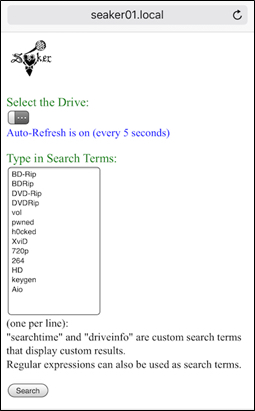
\includegraphics[width=4cm]{images/seaker-hh-screen-2.jpg}
  \caption{Using a browser to connect to {\tt http://seaker01.local}}
  \label{fig:screen-2}
  \end{center}
\end{figure}

(4)~Once any storage media devices that are found at a search warrant scene
are connected to the RP, the investigator will typically wait for a
few minutes (with some times up to 10 minutes for 1Tb disks with
millions of files) for the file list to be built. Searches can then
be carried out very quickly; essentially, \verb|grep| browses the file
list, line by line, outputting those lines that conform to at least
one pattern specified in the ``Type in Search Terms:'' window. Once
this finishes, the investigator will have the results presented as in
Figure~\ref{fig:screen-3}.

The filenames themselves can be incriminating evidence, such as in
Child Pornography (CP) cases, where the material has a commonly used
naming convention, e.g., ``lolita'' which can be found with the grep
pattern \verb|.*lolita.*| (`\verb|.*|' means the
following: `\verb|.|' (period)  matches any single character of any
value, except
a newline, and `\verb|*|' (asterisk) matches zero or more of the
preceding character or expression) or simply \verb|lolita|.
This can be used by the
investigators to question the suspects.  The questioning usually
takes place at the same time as the forensic examiners triage the
evidence, and one of the requirements of \gls{seaker} was to be fast so that
investigators can start getting intelligence quickly from the initial
processing of the scene.

\newpage

\begin{figure}[ht]
  \begin{center}
  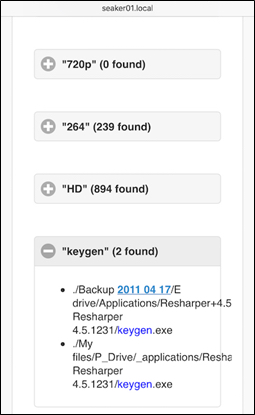
\includegraphics[width=4cm]{images/seaker-hh-screen-3.jpg}
  \caption{The results of the search of a particular device.}
  \label{fig:screen-3}
  \end{center}
\end{figure}

\newpage
(5)~The user process flow is documented in the following
figure~\ref{fig:user_process_flow}.

\begin{figure}[ht]
  \begin{center}
  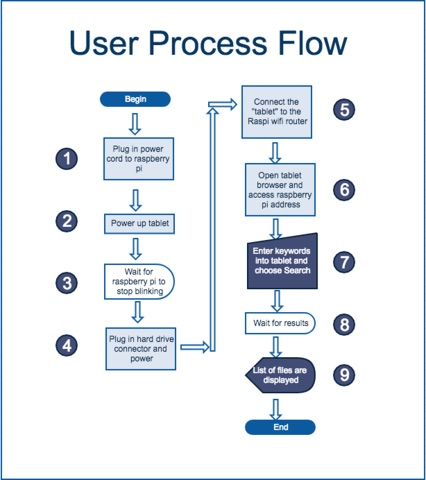
\includegraphics[width=8cm]{images/user_process_flow.jpg}
  \caption{The functionality of \gls{seaker} from the user perspective.}
  \label{fig:user_process_flow}
  \end{center}
\end{figure}

\newpage
\subsection{Code}
\subsubsection{Filename Collection Code (in C)}
\lstinputlisting[language=bash]{code/collect_files.c}

\subsubsection{Maybe other code?}


\newpage
\bibliographystyle{plain}
\bibliography{references}








































\newpage

\section{STOP HERE - Abstract}
\label{sect-abstract}

Goals:
\begin{itemize}
  \item preserve and protect evidenciary integrity
  \item reduce evidence gathering and triage analysis time
  \item prevent adding more to backlog than necessary by preventing over-confiscation
  \item reduce need for on-scene Digital Forensic Ssientists
  \item reduce backlog of digital evidence for tackling backlog
\end{itemize}

\gls{seaker} tradeoffs: Precision (only relevant files) vs Recall (all relevant files)
- level of recall required at triage stage can be sacraficed\\

Introduce online storage system for digital forensic metadata format to enhance sharing capabilities across
jurisdiction boundaries and prevent sharing complexities

\section{Meetings with Frank}
\label{sect-frank}
\vspace{0.5 cm}
\subsection{May 18th, 2018}

My meeting with Frank Lyu, a civilian working for the Ventura County Sherriff's department, on loan to
the Southern California High Tech Task Force (SCHTTF) went well.  The SCHTTF is an 8 person team made up of
four civilians and four deputies, all reporting directly to the Ventura County District Attorney's office.
We met for lunch and I was able to ask him questions about the environment he works in as well as touch on
ranking the high value items that this SEAKER project could provide.\\

First, we talked about his work environment.  He has several responsibilities working for SCHTTF.  The first
and foremost is his caseload, which consists of examining digital evidence using forensic techniques in his
lab that result in a report to the District Attorney's office.  His other responsibilites include assisting
the District Attorney and staff with evaluating defense evidence reports, studying digital forensic 
technologies (for when he has to explain things to juries), helping other agencies identify and catalog
evidence that they are not familiar with, helping serve warrants on critical cases, and helping to retrieve
lost digital materials for other law enforcement agencies.

He explained that following the processes and procedures is by far the most important aspect of his job.  The
evidence handling, storage, and evaluation are critical to whether a case succeeds or is dismissed. Frank
began to describe the intake process, which involves the evidence, the agency report, and the search warrant
that will be used to search and evaluation the materials.  We did not go into further detail.

Items he looks for during an on-site warrant are: user accounts, previewing the materials (especially in
cases involving CP), and checking for the existence of Peer-to-Peer sharing utilities.  In addition, he 
strives to collect the following networking information: publically broadcast SSIDs, each SSID's level of
encryption, how many devices are connected to the router, and the external IP address for the router.

Value of SEAKER in the field: Filename search utilizing regular expression, the networking information 
specified in the last paragraph, producing a report, making an ios app instead of using a webpage, links
for the files found, and clickable thumbnails.

Value of SEAKER in the lab: Filename search utilizing regular expression and SEAKER hashes of images.  He
also mentioned a Microsoft tool called PhotoDNA that they currently use to find naked humans.

I asked about obtaining all of the statistics related to ingestion or evidence, caseload, pace at which
evidence can be evaluated, etc.  Frank's answer was that Adam could probably provide that information
without lab access, but that Michael should be asked to talk to Adam.

Finally, Frank mentioned that sometimes in financial cases, he is asked to search computers at business
offices, and the ability to search for specific filenames is very important there.

\newpage
\section{Background}
\label{sect-background}

\subsection{Introduction to Terms}
\vspace{0.5 cm}
\subsubsection{DEFR and DES Investigation Roles}
\vspace{0.5 cm}
DEFR is Digital Evidence First Responder\\

DES is Digital Evidence Specialiat\\

\subsubsection{Digital vs. Physical Evidence}
\vspace{0.5 cm}
I believe there should be a section here that examines (or at least introduces) the differences and similarities
between regular physical (non-digital) evidence and digital evidence.  Including in the analysis is the metaphore of
how physical evidence is handled (bags, DNA, fingerprints) and how that directly relates to the digital evidence
model.  Contamination must be avoided.\\

\subsubsection{Reactive vs. Proactive Digital Forensic Investigation Processes}
\vspace{0.5 cm}
\textit{Reactive} digital forensic investigation processes are utilized after an offense has been committed to help
identify the charges and suspects.  This is the most common process for digital forensics.  The \textit{proactive}
digital forensic investigation processes are to attempt to detect before or during an active offense is committed.
This is not a job for a typical law enforcement investigator.\\

This research is based on the reactive digital forensic investigation process in the hopes of reducing the digital
forensic lab backlogs across the country and world in two ways.  The first way is to reduce the amount of digital
evidence acquired for the digital forensics lab by enabling efficient and effective on-site triage to occur by
utitizing the commonality of digital evidence collection and analysis into a single step.  The SEAKER digital
evidence triage tool enables an initial collection of information and subsequent searches by any number of local,
on-scene investigators.  These investigators do not need extensive training in digital forensics to utilize it.\\

The second way is to help reduce the existing backlog by enabling a faster, more streamlined approach to initial
potential evidence gathering and reporting.  This approach utilizes the SEAKER digital evidence trial tool to 
perform an initial acquisition and analysis on every exiting case to provide a ``first-look'' at the information.  This
also enables a searching mechanism within a few minutes of plugging in digital evidence media to enable digital 
forensic investigators a quick review of materials.  The process will help with prioritization of evidence, a basic
analysis and potentially initial evidence in the form of a report that can be provided to investigators and
prosecutors.\\

\section{SEAKER Creation}
\label{sect-Creation}

\section{Analysis}
\label{sect-analysis}

\subsection{Process for gathering digital evidence}

First of all, never boot a computer.  That will alter the original state of the hard drive due to the operating
system being loaded.  This may alter the data available for collection and render the digital media ``spoiled'' and
therefore unusable ad evidence in a case.\\

The main point here is to preserve evidentiary integrity and protect against spoilage.\\

Specific training is required to be able to handle digital evidence properly.  What do digital evidence collectors
already have to go through in terms of training?\\

\subsection{SEAKER Usage Methodologies}
\subsubsection{Connected Method}

In this approach, SEAKER is hard-wired using an ethernet cable to the internet or the lab intranet.  The connection
is utilized to connect directly to the Image Hash Storage Server (IHSS) and the Digital Evidence Storage Server (DESS).
The digital evidence is still collected locally, but also being transmitted to the DESS and comparing image hashes
to the IHSS.\\

\subsubsection{Disconnected Method}

In this approach, SEAKER is not connected to an ethernet cable and is solely being used as a wifi router for
collecting digital evidence locally.  A unique digital collection ID will be created when connected to the DESS
at a later time.

\subsection{Automated processes during SEAKER evaluation}

\subsubsection{Local processing}

This section describes the local processing that takes place in both Connected and Disconnected Methods.
\begin{itemize}
  \item picture of digital media
  \item picture of hosting hardward platform (laptop, computer, server, phone, etc)
  \item file list
  \item full log of capturing/viewing/analysis
  \item image thumbnails
  \item video thumbnails
  \item browser history
  \item emails
  \item user profiles
  \item deleted files
  \item image thumbnail subsets (images with faces, bodies, documents, etc)
  \item searches performed
  \item anything ``marked'' as an ``artifact''
\end{itemize}

\subsubsection{Remote processing}

This section describes the remote processing that takes place only when Connected Method is in use.
\begin{itemize}
  \item matching hashes of images
  \item matching hashes of videos
  \item online storage of digital evidence collection for this case at this site and time
\end{itemize}

\newpage
\section{Conclusion and future work}

\subsection{Future work}
\begin{itemize}
  \item Online hard drive investigation (i.e. Cloud Forensics)
  \item Network Traffic Investigation
  \item Video segmentation and video image hashing
  \item crime-specific searchs:
  \begin{itemize}
    \item financial crimes
    \item credit card fraud
    \item hacking
    \item bullying
    \item bloackmail
    \item espianage
    \item fraud
    \item customizable (corporate / military)
  \end{itemize}
  \item OS lockdown (raspbian)
  \item phone specific OS tools
  \item phone specific apps
  \item encrypted devices (password entry location, assessment without password)
  \item running machine RAM assessment
  \item utilize forensics as a service
  \item integrate with Microsoft's photoDNA cloud service
  \item examine local wifi broadcasts
  \item build an iPad app to simpler, more guided use
\end{itemize}

\newpage
\section{Code improvements}
\begin{itemize}
  \item Query Expansion - automatically searching for same query maybe other contexts
  \item Synonym Matching - automatically searching for similar words to query word
  \item collect everything in UTC time
  \item universal way of collecting hard drive hash for verification of evidence integrity
  \item Data Visualizations:
  \begin{itemize}
    \item present all data visualizations for particular drive or all hard drives
    \item graph - size vs amount of files (one hard drive, and all hard drives)
    \item graph - common details (like file type, etc) maybe clickable!
    \item graph/chart - files by date
    \item graph/chart - files by file type
    \item chart - website visits
    \item digital image hashes list (stored and compared)
  \end{itemize}
  \item for analysis: skip OS files, applications files, etc
  \item lock down OS
  \item Investigation Gathering rollup: (stored online)
  \begin{itemize}
    \item Database Schema
    \item metadata
    \item Unique ``gathering ID''
    \item case number
    \item observation report
    \item crime severity
    \item potential offenses
    \item time gathered
    \item gatherer
    \item suspect list
    \item location gathered
    \item suggestions for other research
    \item which computer system it came from
    \item SET of evidence
    \item Digital Evidence item
    \item images of item
    \item unique item ID
    \item file contents
    \item ranking within set of evidence
    \item image thumbnails
    \item collection statistics
    \item etc
  \end{itemize}
  \item swap file review
  \item find encryption Keys 
  \item bulk extractor ? 
  \item thumb strips of movies
  \item predetermine search criteria (passwords, pw, etc)
  \item encrypted password entry?
  \item get file owner, MAC times
  \item sort based on user
  \item sort based on access time
  \item read registry file (make available for search)
  \item time search i.e. time=lastweek, time=5/5/18-5/15/18
  \item internet usage timeline
  \item autosearch/autofilter
  \item email search
  \item for drug search... Spreadsheets, documents, databases, internet purchase strives
  \item for financial search... Spreadsheets, databases, MSMoney, Quicken
  \item CRC of any acquired files (for later integrity comparison)
\end{itemize}

\newpage
\section{Keywords and glossary}
\begin{itemize}
  \item Contraband files
  \item stages: preprocessing, storage, analysis, reporting
  \item stages: gather (document, catalog), triage (analyze, live review, automated review, artifact storage,
  meet threshold?), results (present, graphs, search)
  \item Chain of Custody for digital evidence
  \item Forensic integrity of digital evidence
  \item artifacts = pieces of digital evidence that are of importance to the case
  \item enhanced previewing - better than triage (full drive)
  \item Indecent Image of Children
  \item Image Hash Databases - dbs of digital forensic labs with image hashes
  \item obviate the need for write blockers
  \item early look intelligence gathering
  \item Immediate feedback loop for onsite investigators
  \item ``Suspect's dwelling''
  \item securing a conviction of the offender
  \item protecting future victims
  \item browser artifacts
  \item onsite == in situ
  \item adhere to proven forensic principles
\end{itemize}

\newpage
\section{Graphs, Images, Figures, and tables}
\begin{itemize}
  \item figure - field triage flowchart
  \item figure - each stage field triage flowchart
  \item figure - Image analysis and hash creation flowchart
  \item graph - aquisition time vs full
  \item graph - investigation time vs full
  \item graph - analysis time vs full
  \item graph - total time from initial plug-in to decision to be evidence (threshold)
  \item graph - current backlock in ventura county
  \item figure - DFT vs TCU (Hitchcock\cite{hitchcock2016tiered})
  \item graph - collection time vs number and size of files
  \item figure - see figures in Computer Forensic Field Triage Process model (Rogers)
  \item graph - speed of collecting evidence from same drive based on microSD card used

\end{itemize}

\end{document}

